\chapter{Coordinate Systems and Reference Frames}
\label{ch:coordinate_systems}

\section{Introduction}

Celestial mechanics requires precise specification of positions and velocities. This necessitates well-defined \textit{coordinate systems} (mathematical frameworks for specifying locations) and \textit{reference frames} (physical realizations tied to astronomical objects).

\section{Fundamental Concepts}

\subsection{Inertial vs. Rotating Frames}

\begin{definition}[Inertial Frame]
An \textit{inertial reference frame} is one in which Newton's first law holds: a body not subject to forces moves in a straight line at constant velocity.
\end{definition}

Truly inertial frames don't exist (the universe expands!), but frames fixed relative to distant quasars are effectively inertial for solar system dynamics.

\begin{definition}[Rotating Frame]
A \textit{rotating reference frame} rotates relative to inertial space. Fictitious forces (centrifugal, Coriolis) appear in rotating frames.
\end{definition}

\section{Equatorial Coordinate System}

\subsection{Definition}

The equatorial system uses Earth's equator and rotation axis:

\begin{itemize}
    \item \textbf{Fundamental plane}: Earth's equator (extended to celestial sphere)
    \item \textbf{Primary direction}: Vernal equinox ($\gamma$), where Sun crosses equator northward
    \item \textbf{Pole}: North celestial pole (direction of Earth's rotation axis)
\end{itemize}

\begin{figure}[H]
\centering
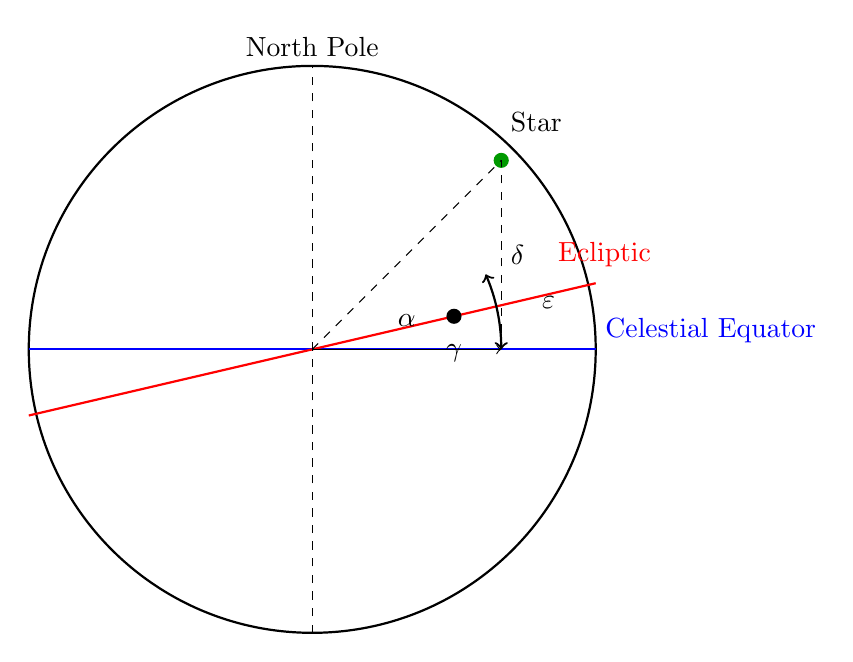
\begin{tikzpicture}[scale=1.2]
    % Celestial sphere
    \draw[thick] (0,0) circle (3);
    
    % Equator
    \draw[thick, blue] (-3,0) -- (3,0);
    \node[blue, right] at (3,0.2) {Celestial Equator};
    
    % Ecliptic
    \draw[thick, red] (-3,-0.7) -- (3,0.7);
    \node[red, right] at (2.5,1) {Ecliptic};
    
    % Vernal equinox
    \fill (1.5,0.35) circle (0.08);
    \node[below] at (1.5,0.15) {$\gamma$};
    
    % Poles
    \draw[dashed] (0,-3) -- (0,3);
    \node[above] at (0,3) {North Pole};
    
    % Obliquity
    \draw[<->, thick] (2,0) arc (0:23.4:2);
    \node at (2.5,0.5) {$\varepsilon$};
    
    % Star position
    \fill[green!60!black] (2,2) circle (0.08);
    \draw[dashed] (0,0) -- (2,2);
    \draw[dashed] (2,0) -- (2,2);
    \draw[->] (0,0) -- (2,0);
    \node at (1,0.3) {$\alpha$};
    \node[right] at (2,1) {$\delta$};
    \node[above right] at (2,2.2) {Star};
\end{tikzpicture}
\caption{Equatorial coordinate system showing right ascension ($\alpha$) and declination ($\delta$). The obliquity $\varepsilon \approx 23.4^\circ$.}
\label{fig:equatorial}
\end{figure}

\subsection{Spherical Coordinates}

Positions are specified by:

\begin{description}
    \item[Right Ascension ($\alpha$)] Angle eastward from vernal equinox along equator ($0^\circ$ to $360^\circ$, or 0h to 24h)
    \item[Declination ($\delta$)] Angle north (+) or south ($-$) of equator ($-90^\circ$ to $+90^\circ$)
    \item[Distance ($r$)] Radial distance from origin
\end{description}

Conversion to Cartesian coordinates:

\begin{align}
x &= r \cos\delta \cos\alpha \\
y &= r \cos\delta \sin\alpha \\
z &= r \sin\delta
\end{align}

\section{Ecliptic Coordinate System}

\subsection{Definition}

The ecliptic system uses Earth's orbital plane:

\begin{itemize}
    \item \textbf{Fundamental plane}: Ecliptic (Earth's orbital plane)
    \item \textbf{Primary direction}: Vernal equinox (same as equatorial)
    \item \textbf{Pole}: Normal to ecliptic plane
\end{itemize}

Coordinates are:
\begin{description}
    \item[Ecliptic Longitude ($\lambda$)] Angle from vernal equinox along ecliptic
    \item[Ecliptic Latitude ($\beta$)] Angle north/south of ecliptic
\end{description}

\subsection{Why Use Ecliptic Coordinates?}

For solar system objects:
\begin{itemize}
    \item Planetary orbits lie near the ecliptic ($|\beta| < 10^\circ$ typically)
    \item Simplifies perturbation calculations
    \item Natural frame for heliocentric dynamics
\end{itemize}

\section{Transformation Between Systems}

\subsection{Ecliptic $\leftrightarrow$ Equatorial}

The transformation involves rotation about the $x$-axis (vernal equinox direction) by the \textit{obliquity} $\varepsilon \approx 23.43929^\circ$:

\begin{equation}
\begin{bmatrix} x \\ y \\ z \end{bmatrix}_{\text{eq}}
= 
\mathbf{R}_x(\varepsilon)
\begin{bmatrix} x \\ y \\ z \end{bmatrix}_{\text{ecl}}
=
\begin{bmatrix}
1 & 0 & 0 \\
0 & \cos\varepsilon & -\sin\varepsilon \\
0 & \sin\varepsilon & \cos\varepsilon
\end{bmatrix}
\begin{bmatrix} x \\ y \\ z \end{bmatrix}_{\text{ecl}}
\end{equation}

For the inverse transformation (equatorial → ecliptic), use $\mathbf{R}_x(-\varepsilon) = \mathbf{R}_x(\varepsilon)^T$.

\subsection{Implementation}

\begin{lstlisting}[style=cpp,caption={Coordinate transformations in AstDyn}]
#include <astdyn/coordinates/ReferenceFrame.hpp>
using namespace astdyn::coordinates;

// Ecliptic to J2000 equatorial
Vector3d pos_ecl(1.0, 0.5, 0.1);  // AU
Matrix3d rot = ReferenceFrame::ecliptic_to_j2000();
Vector3d pos_eq = rot * pos_ecl;

// Equatorial to ecliptic
Vector3d vel_eq(0.01, 0.02, 0.005);  // AU/day
Matrix3d rot_inv = rot.transpose();  // Orthogonal matrix
Vector3d vel_ecl = rot_inv * vel_eq;
\end{lstlisting}

\section{The J2000.0 Reference Frame}

\subsection{Epoch vs. Equinox}

Two temporal concepts are critical:

\begin{description}
    \item[Epoch] The time for which coordinates are specified (affects positions due to motion)
    \item[Equinox] The time defining the orientation of the coordinate axes (affects reference directions)
\end{description}

Example: "Position at epoch 2025.0 in J2000.0 equinox" means the object's location on January 1, 2025, expressed in a coordinate system whose axes are defined by Earth's orientation on January 1, 2000.

\subsection{Precession}

Earth's rotation axis precesses (wobbles) with a period of ~26,000 years due to tidal forces from the Sun and Moon. This causes the vernal equinox to drift westward along the ecliptic at ~50'' per year.

\begin{figure}[H]
\centering
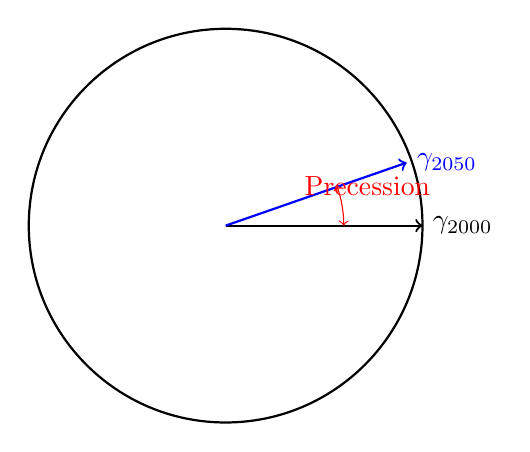
\begin{tikzpicture}
    \draw[thick] (0,0) circle (2.5);
    \draw[thick, ->] (0,0) -- (2.5,0) node[right] {$\gamma_{2000}$};
    \draw[thick, ->, blue] (0,0) -- (2.3,0.8) node[right] {$\gamma_{2050}$};
    \draw[<->, red] (1.5,0) arc (0:20:1.5);
    \node[red] at (1.8,0.5) {Precession};
\end{tikzpicture}
\caption{Precession of the equinoxes over 50 years}
\end{figure}

The J2000.0 frame freezes the equinox at January 1, 2000, 12:00 TT, providing a fixed reference for long-term calculations.

\section{Practical Considerations}

\subsection{Reference Frame Choice}

\begin{itemize}
    \item \textbf{Heliocentric ecliptic}: Natural for planet/asteroid orbits
    \item \textbf{Geocentric equatorial}: Standard for Earth-based observations
    \item \textbf{Barycentric}: Required for precise planetary ephemerides
\end{itemize}

\subsection{Frame Transformations in AstDyn}

The library provides rotation matrices for common transformations:

\begin{lstlisting}[style=cpp,caption={Available transformations}]
// Ecliptic <-> Equatorial (J2000.0)
Matrix3d ecl_to_eq = ReferenceFrame::ecliptic_to_j2000();
Matrix3d eq_to_ecl = ecl_to_eq.transpose();

// ICRS <-> J2000 (small bias correction)
Matrix3d icrs_to_j2000 = ReferenceFrame::icrs_to_j2000();
\end{lstlisting}

More transformations (precession, nutation, GCRS) are available for advanced applications.

\section{Summary}

Key points:
\begin{itemize}
    \item Equatorial system: Tied to Earth's rotation (RA, Dec)
    \item Ecliptic system: Tied to Earth's orbit (natural for heliocentric dynamics)
    \item Transformations: Simple rotation matrices (orthogonal)
    \item J2000.0: Standard epoch/equinox for modern astrometry
    \item AstDyn: Implements all common transformations efficiently
\end{itemize}
